\documentclass[12pt,notitlepage]{article}
\usepackage[bitstream-charter]{mathdesign}
\usepackage{inconsolata}
\usepackage[T1]{fontenc}
\usepackage{microtype}
\usepackage[utf8x]{inputenc}
\usepackage[letterpaper,margin=1in]{geometry}
\usepackage{titlesec}
\usepackage{graphicx}
\usepackage{wrapfig}
\usepackage{caption}
\usepackage{subcaption}
\usepackage{hyperref}

\newcommand\footnoteref[1]{\footnote{\url{#1}}}
\newcommand\tmts[0]{\texttt{tell me to survive}}

\titleformat{\section}{\normalfont\large}{\thesection}{0.5em}{}
\titleformat{\subsection}{\bfseries}{\thesubsection}{0.5em}{}
\titleformat{\subsubsection}{\normalfont}{\thesubsubsection}{0.5em}{}
\titlespacing*{\section}{0em}{0.75em}{0.3em}

\begin{document}
\begingroup
  \centering
  {\Large \texttt{tell me to survive}: Concreteness Fading and Visual
    Programming in Teaching Object-Oriented Programming\\[1em]}

  Andy Jiang, Michael Mauer, and David Li\par
\endgroup

\section{Introduction and Motivation}

Much effort has gone towards methods to teach programming as an
overall concept, with systems like Alice, Scratch, and CodeSpells
demonstrating how visual programming can successfully introduce
students to this field. Our goal is to teach the more specific topic
of object-oriented programming to novice programmers using these same
techniques, focusing on how to abstract and represent ideas such as
method definitions, subclassing, and overriding in such a framework.
Additionally, to reinforce these concepts to an audience already
somewhat familiar with programming, we will introduce concreteness
fading to the system, transitioning students from visual programming
to directly writing code. This will facilitate the learning of these
specific higher-level concepts and abstractions within computer
science, which is important to effectively educate and train the next
generation of computer science and software development students.

\section{Related Work}

The idea of visual programming manipulating robots or other objects in
a virtual world is not a new one; we list several games and projects
in the same vein, with some comparison to our project.

\begin{itemize}
\item CodeSpells\footnoteref{https://codespells.org/}
\item Scratch\footnoteref{https://scratch.mit.edu/}/Alice\footnoteref{http://www.alice.org/}
\item Looking Glass\footnoteref{https://lookingglass.wustl.edu/}
\item Hour of Code\footnoteref{https://code.org/learn}
\item LightBot\footnoteref{https://lightbot.com/hocflash.html}
\item Human Resource Machine\footnoteref{https://tomorrowcorporation.com/humanresourcemachine}
\item Blockly Games\footnoteref{https://blockly-games.appspot.com/}
\item BlockPy\footnoteref{https://github.com/RealTimeWeb/blockpy}
\end{itemize}

CodeSpells, Alice, Scratch, and Looking Glass are more free-form;
instead of specific puzzles or levels to solve, they simply place the
player in a sandbox. Looking Glass tries to come up with metaphors for
object-oriented concepts, and manages to cover more of them than our
project does, but does not employ concreteness fading. Hour of Code,
LightBot, and Human Resource Machine take the same puzzle-oriented
approach our game does, but also lack the concreteness fading
aspect. Blockly Games is the most similar to our approach, initially
using blocks whose labels transition from text descriptions to code,
then changing to a text editor at the end. However, it does not
present a consistent game, changing the theme and mechanics of the
game every few levels. BlockPy is more advanced, enabling the player
to seamlessly switch between code and visual programming (and
translating one to the other), but does not use concreteness fading
either.

\section{Methodology}

\tmts{} is a purely client-side, web-based game built on
HTML5/JavaScript using Python as its instructional language. The core
concept is manipulating robots in a game world via visual or
text-based programming in order to solve puzzles and accomplish
certain objectives.

\subsection{Application Design}

\subsubsection{Concept Progression}

\subsubsection{Concreteness Fading}

Initially, all blocks start off as textual descriptions of
what they do, e.g.\ ``tell \_ to \_'' for method invocation or
``create a new \_ called \_'' for object instantiation (see
\autoref{fig:block-unfaded}). As the player progresses, the labels on
the blocks are faded into actual Python code, as in
\autoref{fig:block-faded}. Eventually, the player will be given a text
editor and asked to write the Python code themselves. Some scaffolding
always remains; for instance, the object hierarchy view always remains
accessible after it is introduced, and serves as a reference for what
classes and methods are available.

\begin{figure}[h]
\centering
\begin{subfigure}{.5\textwidth}
  \centering
  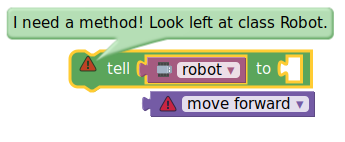
\includegraphics[width=.5\textwidth]{block_unfaded}
  \caption{An unfaded method invocation block.}\label{fig:block-unfaded}
\end{subfigure}%
\begin{subfigure}{.5\textwidth}
  \centering
  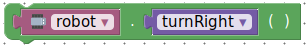
\includegraphics[width=.5\textwidth]{block_faded}
  \caption{The faded method invocation block.}\label{fig:block-faded}
\end{subfigure}
\label{fig:test}
\end{figure}

\subsection{Evaluation}

We evaluated the performance of the game by administering a pre-test
and post-test to all people who completed the game.

\subsubsection{Audience}

We targeted students who are currently enrolled in or have taken only
an introductory programming course. The game was advertised in CS 1110
(Spring 2016) at Cornell, and at <Michael's high school>, as well as
to specific students who have taken CS 1110 here.

\section{Results}

\subsection{Pre- and Post-Test}

\subsection{Subjective Impressions}

\subsection{TODO}

\section{Conclusions}

\end{document}
